\textbf{Неявный алгоритм отслеживания контакта}

% Здесь, как и всюду, будем предполагать, что плоскость колеса вертикальна во все время движения. 
Введем систему отсчета $P{\bf i}{\bf j}{\bf k}$, жестко связанную с колесом (см. рис.~\ref{fig:mecanum}), с началом в его центре $P$. Пусть вектор ${\bf k}$ направлен вдоль оси колеса, ${\bf i}$ и ${\bf j}$ лежат в его плоскости. Введем также две вспомогательные системы отсчета $P{\bf i}_1{\bf j}_1{\bf k}_1$ и $K{\bf i}_2{\bf j}_2{\bf k}_2$, где $K$ -- центр ролика.

Вектор ${\bf i}_2$ направим вдоль оси симметрии ролика, см. рис.~\ref{ContactScheme}. Вектор ${\bf j}_2$ ортогонален ${\bf i}_2$ и лежит в вертикальной плоскости. Третий вектор ${\bf k}_2$ определяется естественным образом как
$$
{\bf k}_2={\bf i}_2\times {\bf j}_2.
$$
% \begin{figure}[hb]
% \centerline{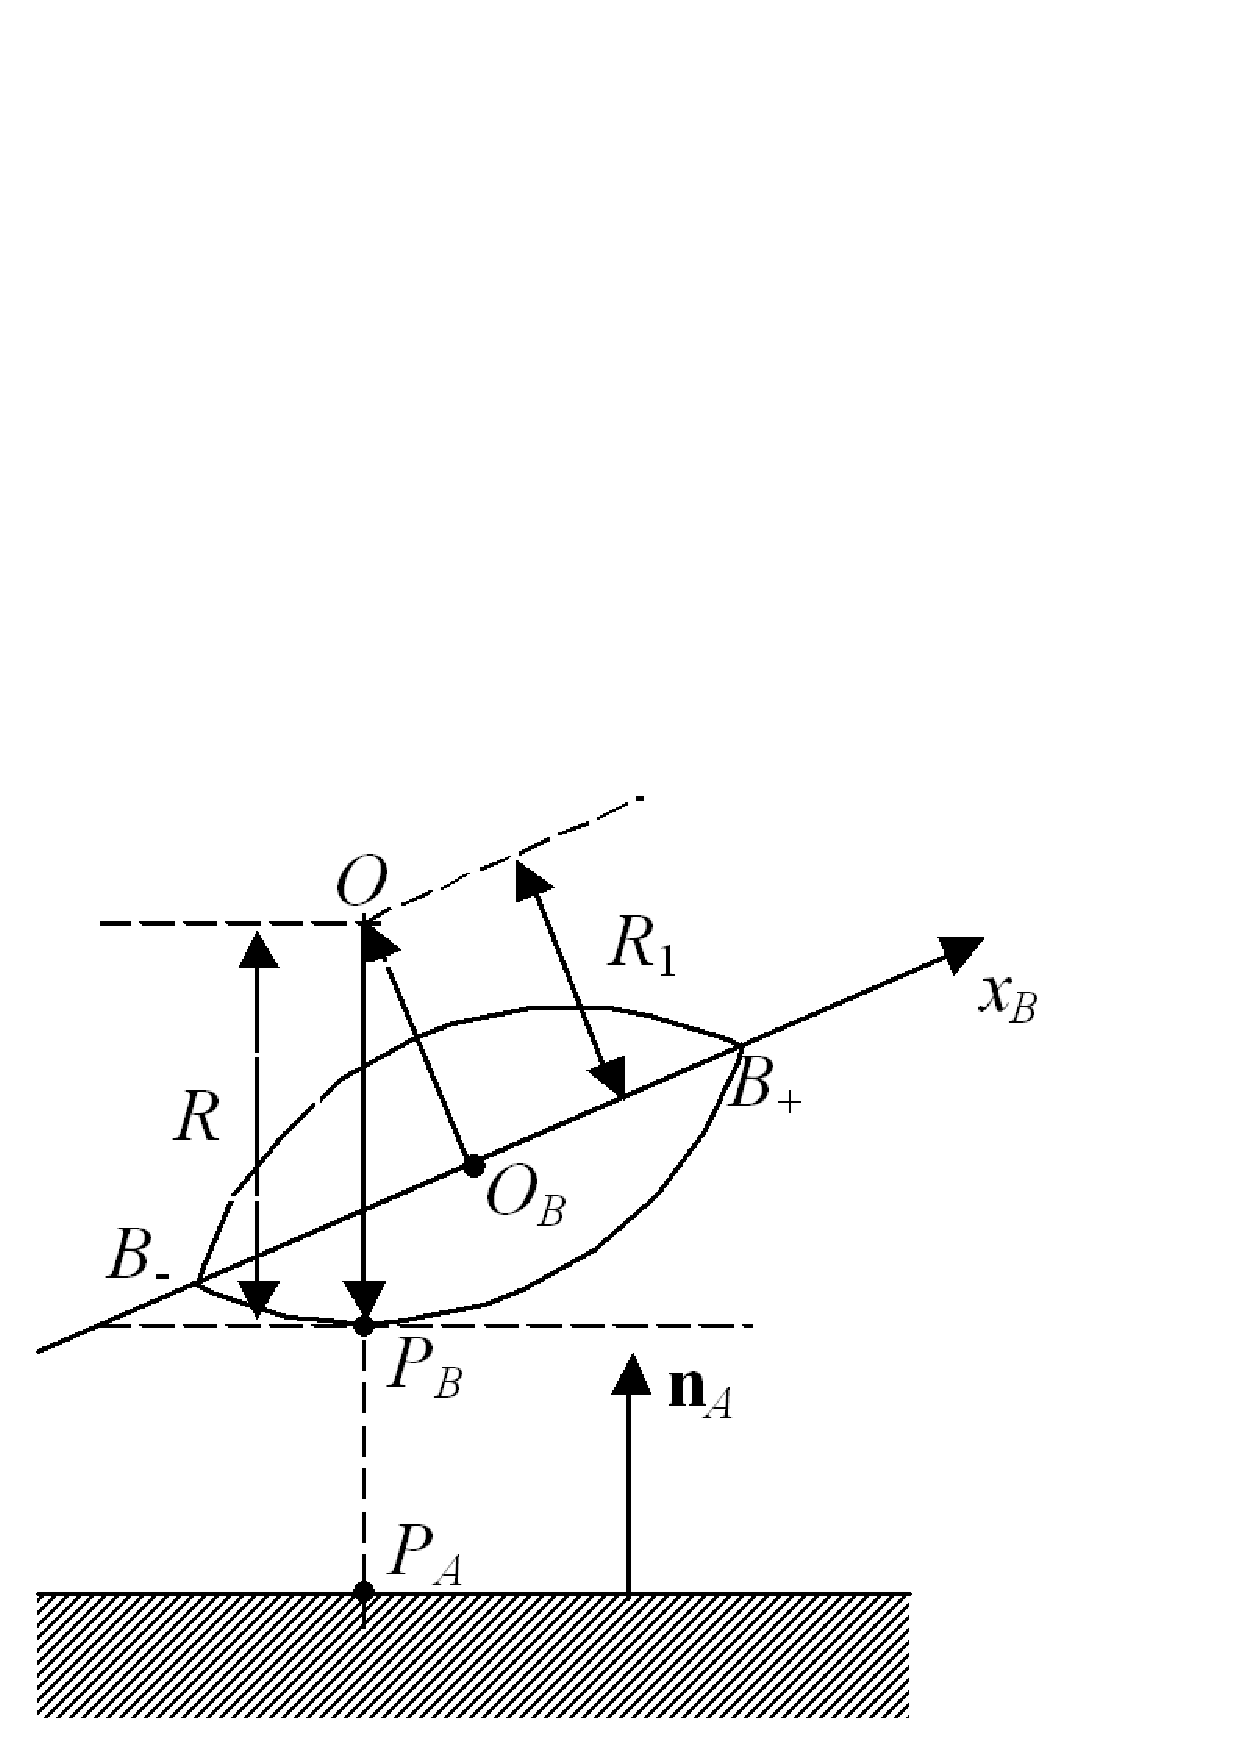
\includegraphics[bb= 0cm 0cm 20cm 17cm,scale=0.30]{RollerSection.png}}
% \caption{Contact tracking scheme.}
% \label{ContactScheme}
% \end{figure}

% Во время счета компоненты всех векторов задаются относительно неподвижной системы отсчета, а положения и ориентации всех тел системы в момент времени $t\in [t_0,t_1]$ считаются известными.

% Таким образом, для системы $K{\bf i}_2{\bf j}_2{\bf k}_2$, имеем:
% $$
% {\bf i}_2=T_B\cdot (1,0,0)^T,\quad\vecrho =
% \left( {\bf r}_{O_A}-{\bf r}_{O_B}\right) /
% \left| {\bf r}_{O_A}-{\bf r}_{O_B}\right| ,
% $$
% где $T_B$ -- матрица ориентации ролика, а единичный вектор $\vecrho$ направлен вдоль луча, выпущенного из центра колеса $O_A$ в сторону центра ролика $O_B$.

Как и в случае $\psi = 0$, определим направление ``на центр колеса'' от центра ролика, т.е. вектор
$$
    \vecrho = \ddfrac
        { {\bf r}_{P}-{\bf r}_{K} }
        {\left| {\bf r}_{P}-{\bf r}_{K} \right|}.
$$

Вектор ${\bf i}_1$ расположим на пересечении плоскости колеса и горизонтальной плоскости. Пусть вектор ${\bf k}_1 = {\bf k}$ ортогонален плоскости колеса и совпадает с одним из векторов базиса, связанного с колесом, и всегда горизонтален. 
% Тогда имеем ${\bf j}_1(t)=(0,1,0)^T$ и ${\bf i}_1(t)={\bf j}_1(t)\times {\bf k}_1(t)$.
$\vec{j}_1$ положим совпадающим с $\vec{\gamma}$. Тогда $\vec{i}_1$ может быть определен как ${\bf i}_1 = {\bf j}_1 \times {\bf k}_1$.

Теперь рассмотрим соотношения, позволяющие вычислить компоненты базисных векторов системы отсчета $K{\bf i}_2{\bf j}_2{\bf k}_2$.

Отметим, что вектор ${\bf i}_2$, направленный вдоль оси ролика, по определению не может принять вертикальное положение, если ролик находится в контакте с опорной плоскостью. Более того, в случае \textit{mecanum} ролик повернут на постоянный угол $\psi > 0$ относительно оси $PK$, и потому во все время движения верно соотношение ${\bf i}_2 \ne \vec{\gamma}$. Таким образом, вектор ${\bf c} = {\bf i}_2 \times \vec{\gamma}$ также отличен от нуля. Положим ${\bf k}_2 = \ddfrac{\vecrho}{|\vecrho|}$. Теперь можно определить ${\bf j}_2$ как ${\bf j}_2 = {\bf k}_2 \times {\bf i}_2$.

Для определения компонент вектора $\vecrho$ воспользуемся кинематическими соотношениями, условиями ортогональности векторов, следующими из определений введенных систем отсчета:
$$
    \vecrho \cdot {\bf i}_2 = 0, \quad \vecrho \cdot {\bf k}_1 = 0,
$$
а точнее, их дифференциальными вариантами:
$$
    \dfrac{d}{dt}\vecrho \cdot {\bf i}_2 + \vecrho \cdot \dfrac{d}{dt}{\bf i}_2 = 0,\quad
    \dfrac{d}{dt} \vecrho \cdot {\bf k}_1 + \vecrho \cdot \dfrac{d}{dt}{\bf k}_1 = 0.
$$

Величина $c_{\beta} = \cos\beta = {\bf i}_2 \cdot \vec{\gamma}$ косинуса угла $\beta$ наклона оси ролика к вертикали $\vec{\gamma}$ также играет важную роль в алгоритме отслеживания контакта. Если текущее значение $c_{\beta }$ меньше некоторого уровня $c_{\beta\max}$, и если одновременно расстояние от центра ролика $K$ до опорной плоскости меньше радиуса колеса $l$, то ролик находится в контакте с опорной плоскостью. В противном случае контакт отсутствует.

Итак, ролик находится в контакте, если только если $\vec{s} \cdot \vec{e}_z < \cos\ddfrac{\pi}{n} $ и $ z_C < l $. В противном случае со стороны опорной плоскости к ролику не приложены силы. В случае контакта, сперва найдем координаты точки ролика, находящейся в данный момент на опорной плоскости:

$$ \vec{r}_C = \vec{r}_K + r\vec{s} - l\vec{e}_z + \lambda\vec{k}_1 $$

Чтобы получить число $\lambda$, умножим последнее уравнение скалярно на ${\bf k}_2$. Отсюда

$$ \lambda = \ddfrac{\left(r\vec{s} - l\vec{e}_z\right)\cdot\vec{k}_2}{ \vec{k}_1\cdot\vec{k}_2} $$
$$ \vec{v}_C = \vec{v}_K + [ \vec{\omega}_{\text{рол}}, \overrightarrow{KC} ],$$

поскольку ${\bf r}_{C}-{\bf r}_{K}$ лежит в вертикальном сечении осесимметричной поверхности ролика, и вектор ${\bf k}_2$ по построению ортогонален этому сечению. В результате радиус-вектор ${\bf r}_{C}$ точки контакта определяется однозначно.

% На рис.~\ref{ContactScheme} также легко видеть, что координаты точки $C$ контакта ролика и плоскости даются выражением
% $$
% {\bf r}_{P_B}={\bf r}_{O_B}+R_1\vecrho -R{\bf j}_1+\mu {\bf k}_1,
% $$
% где число $\mu$ требуется вычислить (см. рис.~\ref{fig:mecanum}). Здесь величина $R_1$ равна расстоянию между точками $O_A$ и $O_B$.